\chapter{UNIXフィルシステム}
ファイルシステムの事例として\emph{UFS(UNIX File System)}を紹介する.
UFSはUNIXで使われてきたファイルシステムを指し様々なバージョンがある.
階層構造のディレクトリシステムを持ち,
マルチユーザで使用できるファイルシステムである.
ここでは,UFSの概念が分かりやすいように,
UFSの特徴を表す仕組みを特定のバージョンに拘らずに紹介する\footnote{
ここで説明していることの多くは概念である.
実際の構造はバージョンによっては全く異なる場合もある.}.

%============================================================================
\section{概要}
UFSは,
1979年にリリースされた Version 7 Unix のファイルシステムと,
それを改良した多くのファイルシステムである.
第\ref{fileSystemConcepts}章では,
木構造のディレクトリシステム,
ハードリンク,
シンボリックリンク,
ボリュームをマウントする方式,
ファイルの属性,
ファイルシステムの操作等で「UNIXの場合」を基本に解説を行ったが,
「UNIXの場合」とは「UFSの場合」であった.

また,WindowsのNTFS,macOSのHFS+やAPFS,
Linuxのext3やext4等のファイルシステムは,
ハードリンクや,ファイル名の大小文字の区別,
アクセス権限等で,
UFSと同じ構造を持っているようにユーザに見せることができる.

%============================================================================
\section{ボリューム内部の配置}
\label{ufsVolumeLayout}
UFSボリューム(パーティション)の内部は,
例えば\figref{ufsVolume}のような配置になっている.
この例は,1セクタ512バイト,1ブロック16セクタ(8KiB),
\inode サイズ128バイトのものである.

\begin{myfig}{btp}{UFSボリュームの構造}{ufsVolume}
  \centering{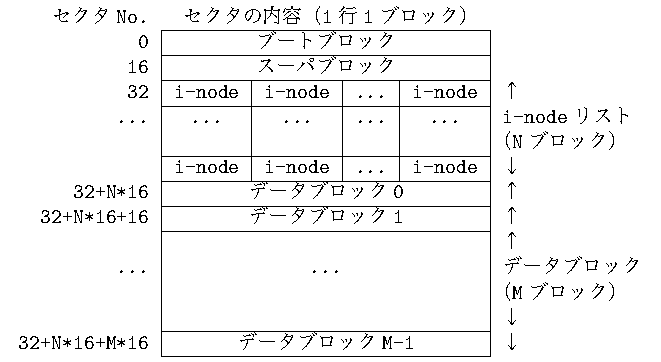
\includegraphics[scale=1.0]{Fig/ufsVolume.pdf}}
\end{myfig}

\begin{itemize}
\item \emph{ブートブロック}\\
  ブートプログラムが格納される.
  PCの場合,ブートブロックのブートプログラムは,
  MBRのブートプログラムによってロード実行される.
\item \emph{スーパーブロック}\\
  ボリュームのサイズ,ブロックのサイズ,\inode リストのサイズ等,
  ファイルシステムを初期化した時に決めたパラメータや,
  最終変更日時,最終マウントポイント,空きブロック数
  等の運用中に変更される値が格納される.
  「ファイルシステムが正常にアンマウントされた」印\footnote{
    「\ref{unmountFlag}一貫性チェック」で紹介した.
  }もスーパーブロックに含まれる.
\item \emph{\inode リスト}\\
  \figref{ufsVolume}の例では,
  128バイトの\inode を512バイトのセクタに4個格納できる.
  16セクタのブロックには$4 \times 16 = 64$個の \inode が格納できる.
  Nブロックの \inode リスト領域全体で$N \times 64$個の\inode が格納される.
  1つの\inode が1つのファイルを管理するので,
  初期化時に決定した\inode リストの大きさによって,
  このファイルシステムに作成できるファイルの最大数が決まる.
\item \emph{データブロック}\\
  ファイルのデータ本体を格納する領域である.
  データブロック領域全体では$M \times 16$セクタを使用している.
\end{itemize}

%============================================================================
\section{\inode (index node)}
1つの \inode が1つのファイルを管理する.
\figref{ufsInodeAndDataBlock}に\inode の構造を簡単に表したものを示す\footnote{
  \figref{ufsInodeAndDataBlock}は,FreeBSD4のソースコード
  \url{https://github.com/freebsd/freebsd/blob/stable/4/sys/ufs/ufs/dinode.h}
  を参考に,一部を簡単化して描いた.
}.

\begin{myfig}{btp}{\inode の構造}{ufsInodeAndDataBlock}
  \centering{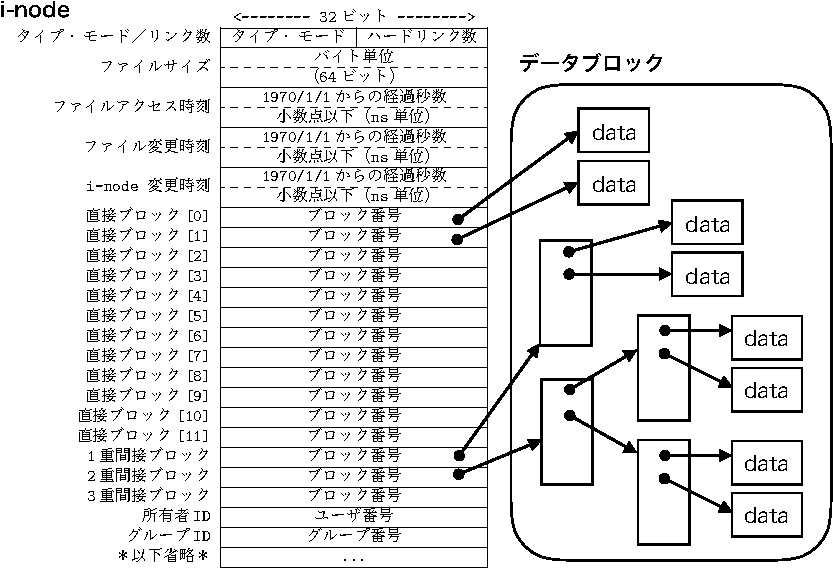
\includegraphics[scale=1.1]{Fig/ufsInodeAndDataBlock-crop.pdf}}
\end{myfig}

\begin{itemize}
\item \emph{タイプ・モード}\\
  タイプ・モードは\|type/sst/rwxrwxrwx|の16ビットから構成される.
  \|type| 4ビットでファイルの型を表現する.
  ファイルの型には,通常ファイル,ディレクトリ,シンボリックリンク,
  キャラクタ型デバイス,ブロック型デバイス,パイプ,ソケット等がある.

  \|ss|の2ビット(Set-uid,Set-gid)はファイルに格納されたプログラムが,
  ファイル所有者やグループの権限で実行されることを表す.
  例えばmacOSの\|/bin/ps|プログラムは,
  プロセス情報を収集するためにシステム管理者の権限で実行される必要があるので,
  これら2ビットが$10_2$に設定されている\footnote{
    macOSで\texttt{ls -l /bin/ps}を実行すると
    ファイルのモードが\texttt{-rwsr-xr-x}のように表示される.
    これは,psプログラムが
    ファイルの所有者の権限で実行されることを表している.}.
  \|t|ビットはOSによって解釈が異なるので,ここでは解説しない.
  \|rwxrwxrwx|の9ビットは,おなじみのファイルの保護モードである.

\item \emph{リンク数}\\
  リンク数はファイルが幾つ名前を持つか(ハードリンクされているか)
  管理するカウンタである.
  リンクを削除しリンク数が 0 になった時にファイルが削除される
  (\inode が解放される).

\item \emph{ファイルサイズ}\\
  ファイルのサイズをバイト単位で表現する.
  \figref{ufsInodeAndDataBlock}の例ではファイルサイズは64ビットである.

\item \emph{3つの時刻}\\
  ファイルの最終アクセス時刻,変更時刻,\inode 変更時刻が記録される.
  各時刻は,次の2つの32ビット整数で表現する.
  1つ目の32ビット整数で1970年1月1日午前0時(UTC)からの経過秒数が表現される
  \footnote{32ビットの経過秒数は2038年にオーバーフローする(負の数になる).
    UNIX時間の2038年問題と言われる.}.
  2つ目の32ビット整数は秒の小数点以下をナノ秒単位で表現する.

\item \emph{直接ブロック}\\
  ファイル本体のデータを格納した12個のデータブロックの番号である.
  \figref{ufsInodeAndDataBlock}はブロック番号が32ビットの例である.
  データブロックサイズが\figref{ufsVolume}のように8KiBとすると,
  最大で$8KiB \times 12 = 96KiB$のファイルまでを表現できる.
  ファイルの第$0$バイトから第$96Ki - 1$バイトまでは,
  いつも直接ブロックで管理される.

\item \emph{1重間接ブロック}\\
  直接ブロックだけでは表現できない大きなファイルに用いる.
  ここに番号を格納したデータブロックを間接ブロックと呼び,
  他のデータブロックの番号を格納するために使用する.

  1ブロックが$8KiB$,ブロック番号が32ビット(4バイト)と仮定すると,
  1つの1重間接ブロックに$8KiB \div 4B = 2Ki$個のブロック番号が格納できる.
  2Ki個のデータブロックでは$8KiB \times 2Ki = 16MiB$のデータを記録できる.
  ファイルの第$96Ki$バイトから第$96KiB + 16MiB - 1$バイトの範囲が,
  1重間接ブロックで管理される.

\item \emph{2重間接ブロック}\\
  1重間接ブロックでも表現できない大きなファイルに用いる.
  ここに番号を格納したデータブロックを2重間接ブロックと呼び,
  1重間接ブロックのブロック番号を格納する.

  1ブロックが$8KiB$,ブロック番号が32ビットと仮定すると,
  1重間接ブロックを用いて$16MiB$のデータを記録できた.
  2重間接ブロックを用いると1重間接ブロックを2Ki個格納できるので,
  $16MiB \times 2Ki = 32GiB$のファイルデータを管理できる.

\item \emph{3重間接ブロック}\\
  2重間接ブロックを2Ki個管理できるので,
  $32GiB \times 2Ki = 64TiB$のデータを管理できる.

\item \emph{所有者ID}\\
  ファイル所有者のユーザ番号を格納する.(マルチユーザに対応)

\item \emph{グループID}\\
  ファイルのグループ番号を格納する.
\end{itemize}

\inode がデータブロックを管理する方式を\emph{インデクス方式}と呼ぶ.
ランダムアクセスをする場合,
インデクス(直接ブロック,間接ブロック等)から素早く目的の
データブロックを見つけることができる.
(リスト方式ではブロックを順に調べる必要があった.)

「システム内には小さなファイルが多く大きなファイルは少ない」
との仮定が成立てば,小さなファイルを効率よく扱えるこの方式は合理的である.
間接ブロックを用いる大きなファイルの場合は少し効率が悪くなるが,
使用頻度が低いので我慢できる.
平均的なファイルサイズは時代によりシステムにより大きく変化するので,
ファイルシステム初期化時にデータブロックサイズを適切に決める必要がある.

内容が全て\|0x00|のデータブロックは割り付けを省略しても良い.
また,ランダムアクセスで途中を飛ばしてデータを書き込んだ場合,
途中のデータが書き込まれたことがないデータブロックも省略できる.
このような途中に穴が空いたファイルのことを
\emph{スパースファイル(sparse file)}と呼ぶ.
スパースファイルはデータブロックを消費しないで広いアドレス空間を提供できる.

%============================================================================
\section{ディレクトリファイル}
ディレクトリファイルは
\inode の\|type|が\emph{ディレクトリ}になっているファイルである.
ディレクトリファイルのデータブロックには,
ファイル名と\inode の対応表が記録される.
対応表の1行をディレクトリエントリと呼ぶ.
ディレクトリエントリは,
\figref{ufsDirEntry}に示す可変長のものである\footnote{
\figref{ufsDirEntry}は,FreeBSD4のソースコード
\url{https://github.com/freebsd/freebsd/blob/stable/4/sys/ufs/ufs/dir.h}
を参考に描いた.
}.
エントリの各フィールドの意味は次の通りである.

\begin{myfig}{btp}{ディレクトリエントリの構造}{ufsDirEntry}
  \centering{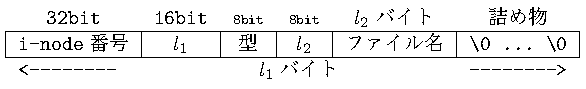
\includegraphics[scale=1.0]{Fig/ufsDirEntry.pdf}}
\end{myfig}

\begin{itemize}
\item  \emph{\inode 番号}は,
  ファイル名とリンクされるファイル本体の\inode 番号である.
\item \emph{$l_1$}は,
  ディレクトリエントリの長さをバイト単位で表す.
  $l_1$は4の倍数でなければならない.
\item \emph{型}はファイル本体の型を格納する.
  また,エントリが削除された時,空エントリを表現する値%(\|DT_WHT|)
  を格納する.
\item \emph{$l_2$}は,
  ファイル名の長さをバイト単位で表す.
  $l_2$が8ビットなので,ファイル名は255バイト以内に制限される.
\item \emph{ファイル名}は,
  $l_2$バイトのファイル名を格納する領域である.
\item \emph{詰め物}には,
  ディレクトリエントリの長さが4の倍数になるように\|0x00|のバイトを書き込む.
\end{itemize}

%============================================================================
\section{パス名と\inode の対応付け}

以下ではOSが\|/etc/passwd|ファイルを探索する手順\footnote{
  例えば\texttt{open}システムコールが,
  渡されたパス名をもとに目的ファイルを探索する手順のこと.
}を\figref{ufsSample}を用いて説明する.

\begin{myfig}{btp}{UFSで\texttt{/etc/passwd}ファイルを探索する手順}{ufsSample}
  \centering{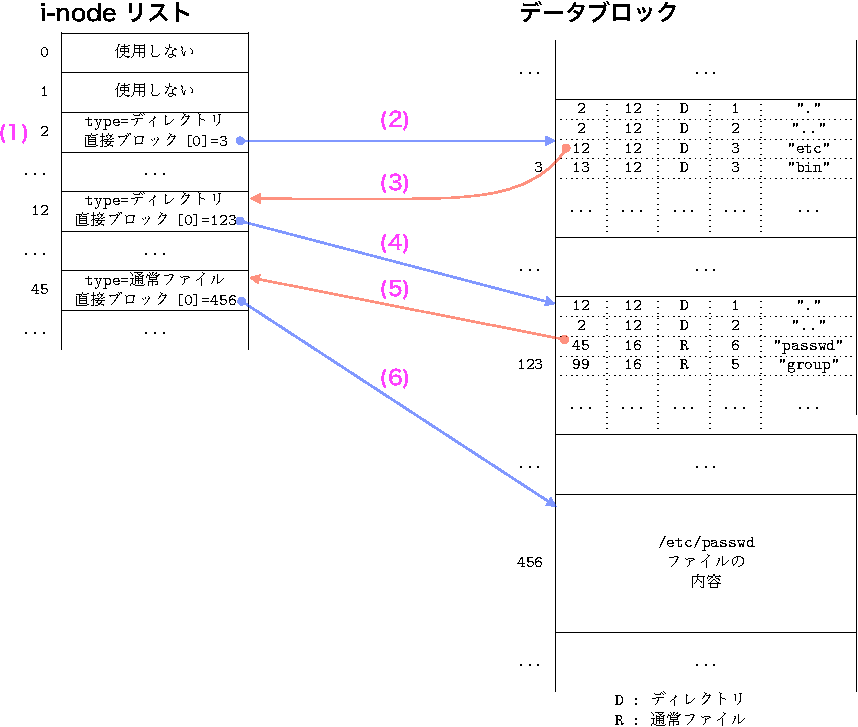
\includegraphics[scale=1.1]{Fig/ufsSample-crop.pdf}}
\end{myfig}

\begin{enumerate}
\item[(1)] パスは絶対パスなのでルートディレクトリから探索を開始する.
  この例では,
  ルートディレクトリの\inode 番号は必ず2と決められているものとしている.
\item[(2)] ルートディレクトリの\inode から,
  データブロック3にルートディレクトリの内容が格納されていることが分かる.
  データブロック3を見に行く.
\item[(3)] データブロック3に格納されているディレクトリエントリを
  解析する\footnote{
    ディレクトリファイルには\texttt{.}や\texttt{..}も
    格納されていることも確認して欲しい.
  }.
  ファイル名\|etc|は3番目のエントリに見つかる.
  このエントリから,12番の\inode が\|etc|に対応することが分かるので,
  \inode リストの12番目のエントリを見に行く.
\item[(4)] 12番目の\inode から\|etc|はディレクトリファイルであること,
ディレクトリファイルの内容がデータブロック123に格納されていることが分かる.
データブロック123を見に行く.
\item[(5)] データブロック123に格納されているディレクトリエントリを解析する.
  ファイル名\|passwd|は3番目のエントリに見つかる.
  このエントリから,45番の\inode が\|passwd|に対応することが分かるので,
  \inode リストの45番目のエントリを見に行く.
\item[(6)] 45番目の\inode から\|passwd|は普通のファイルであること,
  ファイルの内容がデータブロック456に格納されていることが分かる.
  データブロック456を読みに行く.
\end{enumerate}

%============================================================================
\section{まとめ}
UFSは,Version 7 Unix のファイルシステムと,
それを改良した多くのファイルシステムのことを指す.
様々な改良がされた多数のバージョンが存在する.
また,WindowsのNTFS,macOSのHFS+やAPFS,
Linuxのext3やext4等のファイルシステムはUFSではないが,
ハードリンクを始め,
本書で説明したUFSと同じ構造であるような振る舞いをすることができる.

この章では,
UFSボリュームの構造は概念のみを示し,
\inode とディレクトリエントリはFreeBSD4を
参考にフォーマットを示し内容を解説した.
最後に,UFS上でパスを解析し特定のファイルを見つける手順を,
例を用いて説明した.

%==============================================================================
\newpage
\section*{練習問題}
\begin{enumerate}
\item 次の言葉の意味を説明しなさい.
  \begin{itemize}
  \item ブートブロック
  \item スーパーブロック
  \item \inode
  \item \inode リスト
  \item インデクス方式
  \item スパースファイル
  \item ディレクトリファイル
  \item ディレクトリエントリ
  \item 直接ブロック
  \item 間接ブロック
  \end{itemize}

\item ブロックサイズが8セクタ(4KiB)の場合,
  直接ブロックだけ用いて表現できるファイルの最大サイズを答えなさい.

\item ブロックサイズが8セクタ(4KiB)の場合,
  1重間接ブロックを用いることによって,
  直接ブロックだけの場合と比較して,
  ファイルサイズを最大でどれだけ大きくできるか答えなさい.

\item ブロックサイズが8セクタ(4KiB)の場合,
  2重間接ブロックを用いることによって,
  直接ブロックと1重間接ブロックだけ使用する場合と比較して,
  ファイルサイズを最大でどれだけ大きくできるか答えなさい.

\item \figref{ufsInodeAndDataBlock}の例がスパースファイルを表現しているとする.
  また,ブロックサイズ等は「\ref{ufsVolumeLayout}ボリューム内部の配置」で
  示したものと同じとする.
  次のアドレスはデータブロックが割り当てられいるか答えなさい.

  \begin{enumerate}
    \item 第\|0x00000000|バイト
    \item 第\|0x00001000|バイト
    \item 第\|0x00010000|バイト
    \item 第\|0x00100000|バイト
    \item 第\|0x01000000|バイト
    \item 第\|0x10000000|バイト
  \end{enumerate}

\end{enumerate}
